
%- Preliminaries

\chapter[ADAPTIVE SUBMODEL SELECTION IN HYBRID MODELS]{Adaptive submodel selection in hybrid  models}\label{adaptiveselection}

\WeAreOn{\cthree}
\typeout{Chapter 3: Prologue to the paper}
\section{Prologue to the paper}  
This chapter is a (verbatim) paper that I was invited to submit for a special topic
issue of the refereed journal \emph{Frontiers in Environmental Science}. The
issue's intent was to focus attention on hybrid models which couple
component-models (submodels) from across the range of modelling
paradigms, and to encourage the development of this sort of model in
the context of ecological research.  The paper develops a thought
model which demonstrates a high level mechanism for governing the mix
of representations used in the model based on the state of the system
and the states of its components.

Simple rules can be used to govern transitions from one representation
to another (Chapter \ref{modelefficiency}), but these local
transitions may degrade the quality of the simulation as a whole. The
biomass of grass a farm's paddocks is probably quite
adequately represented by a single number if there is little or no
grazing, but with more livestock we might need to represent each
paddock's biomass individually, \ldots and possibly each paddock as a
finely resolved field showing where the animals graze most intensely.

The appendix to the paper is an early version of the mathematical
machinery developed in Chapter \ref{treering}. Since publication, the
basic mathematical structure has changed significantly --- this early
version is much harder to manipulate, and generally less powerful.
The propositions and assertions in this chapter are presented largely
without proof, though the corresponding propositions are proved for
the material in Chapter \ref{treering}.

\pagebreak
\typeout{Chapter 3: Adaptive submodel selection in hybrid  models}
\section*{Adaptive submodel selection in hybrid  models}

\begin{center}
  Randall Gray\footnote{{Published in \emph{Frontiers in Environmental Science}, 20/8/2015}\\
    Corresponding author:\texttt{Randall.Gray@limnal.net} (Randall Gray),\\
      \texttt{Simon.Wotherspoon@utas.edu.au} (Simon Wotherspoon)
      }

    \emph{University of Tasmania}

    Simon Wotherspoon 

    \emph{University of Tasmania}
\end{center}

\rule{\textwidth}{2pt}

\begin{description}
  \item[ ]
    \textbf{Abstract}

     Hybrid modeling seeks to address problems associated with the
     rep\-re\-sen\-ta\-tion of complex systems using ``single-paradigm'' models:
     where traditional models may represent an entire system as a
     cellular automaton, for example, the set of submodels within a hybrid
     model may mix rep\-re\-sen\-ta\-tions as diverse as in\-di\-vidu\-al-based models
     of organisms, Markov chain models, fluid dynamics models of regional
     ocean currents, and coupled population dynamics models. In this
     context, hybrid modelers try to choose the best rep\-re\-sen\-ta\-tions for
     each component of a model in order to maximize the utility of the
     model as a whole.

     Even with the flexibility afforded by the hybrid approach, the set
     of models constituting the whole system and the dynamics associated
     with interacting models may be most efficient only in parts of the
     global state space of the system.  The immediate consequence of this
     possibility is that we should consider adaptive hybrid models whose
     submodels may change their rep\-re\-sen\-ta\-tion based on their own
     state and the states of the other sub\-models within the system.

     This paper uses a simple example model of an artificial ecosystem to
     explore a hybrid model which may change the form of its component
     sub\-models in response to their local conditions and internal state
     relative to some putative optimization choices.  The example
     demonstrates the assessment and actions of a ``monitor'' agent which
     adjusts the mix of sub\-models as the model run progresses.  A simple
     math\-e\-mat\-\i\-cal structure is also described and used as the basis for a
     sub\-model selection strategy, and alternative approaches are briefly
     discussed.
\end{description}

\rule{\textwidth}{2pt}



%- Beginning of text

%-- Introduction
\typeout{Chapter 3: Introduction}
\section{Introduction}
%----> The case has been made <----
The case has been made for developing systems with sub\-models that
change their rep\-re\-sen\-ta\-tion according to their state.
\citet{vincenot2011theoretical} identify reference cases describing the
major ways system dynamics models (\SD) and in\-di\-vidu\-al-based models
(\IB) can be coupled. Their final case, \SD-\IB\ model swapping, is
exemplified in the models described by both \cite{bobashev2007hybrid}
and \cite{Gray2012adaptive}. These papers argue that we can improve on
conventional hybrid models, in terms of efficiency, fidelity, model
clarity or execution speed by using an approach that allows the
sub\-models themselves to change during a simulation. The last two
papers implement simple models which demonstrate the approach, with
correspondingly simple mechanisms to control transitions between
different sub\-models. 

%----> way to increase fidelity  <----
Some authors argue that the explicit coupling of \SD\ models and
\IB\ models may provide greater clarity and resolution in modeling
\citep{vincenot2011theoretical,Fulton2010approaches}: parts of a model that are
most clearly the result of aggregate processes are likely to be better
suited to modeling with a \SD\ approach. In contrast, the
parts of a system where in\-di\-vidu\-als have a significant influence on
their neighbors \citep{botkin1972some} are better suited to an
\IB\ approach. This argument is closely tied to the notion of model
fidelity. Following \cite{delsole2010model}, we take
\emph{fidelity} to be the degree to which a model's trajectory is
compatible with real trajectories.  If our immediate goal is to
maximize the utility of the set of sub\-models within a model
as it runs, this must include the fidelity of the system in the
decision process.

%----> Fidelity is harder to measure than speed or error  <----
Measuring or estimating execution speed and numerical error are
comparatively straight-forward, but determining model fidelity is not.
Models with a high degree of fidelity should produce results which are
consistent with observed data from real instances of the system they
model across both a wide range of starting conditions and under the
influence of ad hoc perturbations, such as fires through a forested
domain. Model fidelity is addressed by \cite{delsole2010model} in the
context of seasonal forecasting models. They explore the relationship
between fidelity and skill using an information-theoretic approach.
They describe \emph{skill} loosely as the ability to reproduce actual
trajectories, and they describe \emph{fidelity} as measuring the
difference between the distribution of model results and the
distribution of real world results.  They highlight the attractiveness
of mutual information and relative entropy as measures (or at least
indices) of skill and fidelity, but they observe that in their domain,
climate modeling, the necessary probability distributions are unknown.

%----> fidelity w.r.t. cost & benefit <----
The issues of fidelity and the attendant cost/benefit balance are
central to the dis\-cus\-sion in \cite{bailey1992scientific}.  This paper
assesses the costs and benefits of three dif\-fer\-ent upgrades to an
existing model designed to help de\-ter\-mine the best mix of types of
radios used in a mil\-i\-tary con\-text; their ob\-jec\-tive is to prioritize
im\-ple\-men\-ta\-tion of the refinements of their model. The fun\-da\-men\-tal
issues they address are substantially the same as issues that
in\-flu\-ence dynamic model selection.

%----> Boiler optimization, win for fidelity <----
The paper by \cite{yip2004effect} compares three models used for
real-time optimization of a boiler network: simple linear
extrapolation from the system's current state, quadratic prediction
with the coefficients based on historical data and updated at every
step, and a detailed process model that corresponds closely with the
physical elements of the modeled system. Their conclusion correlates
the fidelity of the model with its ability to control the real-time
optimization of the system. They explicitly note that there are real
costs associated with the increased fidelity. These costs include
model development and the need for more expensive sensors. They note
that increasing fidelity in the model enabled the system to adapt to
changing fuel more efficiently, and that when there were frequent
changes in fuel characteristics the simpler models performed poorly.

The projects described in \cite{Little2006nws} and \cite{Fulton2011ningaloo}
both used hybrid models as a means of decreasing the run-time, and
increasing the fidelity of the modeled contaminant uptake in 
simulated organisms. This was accomplished by mixing in\-di\-vidu\-al-based
sub\-models and regional population-based systems
models. \cite{Gray2012adaptive} explicitly used changes in the rep\-re\-sentation
of agents to improve the execution speed of a contamination tracking
model, without losing the fidelity of the in\-di\-vidu\-al based uptake
model. In this paper we will develop a more general strategy which may
be appropriate for more complex systems.


\typeout{Chapter 3: Model organization}
\section{Model organization}

For clarity, we will take the term \emph{niche} to refer to something
in the model which could be modeled in several ways: a ``porpoise''
niche could be filled by many instances of an in\-di\-vidu\-al-based
model, models of pods, or a regional \SD\ model of the porpoises.
This is essentially the same as the term \emph{component} in
\cite{vincenot2011theoretical}. The motivation for departing from this
convention arose from confusion resulting from inadvertently using
\emph{component} both in a technical and non-technical sense.  The
close analogy between the nature of a niche in an ecosystem and the
nature of a component as discussed in \cite{vincenot2011theoretical}
suggested the choice of \emph{niche}. 

Each of the alternative ways of representing a niche can be viewed as
a \emph{sub\-model}, and the word \emph{rep\-re\-sen\-ta\-tion} will
be used to reflect a particular choice of sub\-model within a niche.
An explicit instance of a sub\-model (such as a specific pod or an
\SD\ model) will be referred to as an \emph{agent}.  The
\emph{con\-fig\-ur\-a\-tion} of the model at any moment consists of
the particular set of sub\-models which fill the niches that comprise
the model as a whole. For an adaptive hybrid model, there may be a
large number of possible con\-fig\-ur\-a\-tions and the selection of a
``best'' con\-fig\-ur\-a\-tion is a complex matter.

Each agent running in a model must necessarily have data which can
serve to characterize it for these assessments. This data would
typically be some subset of its state variables, but the data alone
may not be enough to base an assessment on: there may also be
extrinsic data which play a role in a particular sub\-model's or agent's
activity and impinges on its suitability. Then, the characterization
of an agent --- its \emph{state vector} --- is an amalgam of its own
state and the state of other niches it interacts with, and it can be
regarded as a point in the state space which the sub\-model is defined
over. 

A corresponding set of data characterizes a niche in the model; here,
it is typically some appropriate aggregation of agent-level state
variables (a biomass-by-size distribution, for example), relative
rankings of the suitability of agents and alternative sub\-models, and
indications of what extrinsic support all of the various alternatives
require. This niche-level state vector provides the data needed for
optimizing the con\-fig\-ur\-a\-tion globally,
and for managing the con\-fig\-ur\-a\-tion when niche-wide effects
become significant, for example, for an incipient epidemic.

Thus, there are three distinct levels of organisation which may
influence the considerations regarding the current configur\-ation, and
inform any decision about what may need to change, namely
\begin{enumerate}
\item agent-level data need to be examined to determine how well
  suited each agent is to its current state and the context provided
  by the agents it interacts with,
\item a niche-level assessment which compares the utility of each of
  its current agents within a niche with their alternative sub\-models,
  and
\item a model-wide assessment which determines whether there are
  cross-agent conflicts or unmet needs arising from a particular
  con\-fig\-ur\-a\-tion.
\end{enumerate}

The state vectors which form the domains of sub\-models and niches are
loci in appropriate state spaces and can be encoded as an elements in
appropriate vector spaces. The math\-e\-mat\-i\-cal tools to manipulate these
state vectors can then be applied to calculate the distances between
two states, the similarity of loci which represent models or niches,
or to identify trends or clusters.



\subsection{Implications of changing con\-fig\-ur\-a\-tions}

At a basic level, hybrid models are designed to represent entities or
processes in the real world in a way which brings more clarity,
efficiency, or fidelity that may be possible with more traditional
approaches. Adaptive hybrid models, implicitly acknowledge that the
appropriate rep\-re\-sen\-ta\-tion may change through time. An important
consequence is that when a sub\-model in a niche changes, it may trigger
changes in rep\-re\-sen\-ta\-tion elsewhere in the model.

We might consider an example where an \SD\ sub\-model which represents
the prey for an \SD\ based predator changes to \IB\ sub\-models. It
seems reasonable to expect the rep\-re\-sen\-ta\-tion of the predator might
follow suit. This may change the spatial resolution, the fineness of
the ``quantities'' represented, and possibly the time steps associated
with the predators and prey. Disparities in either of the first two
are simple enough to deal with: modelers routinely use interpolation
as a means of removing inappropriate edges, or generating subscale
data, for example.  Changes in an agent's time step can have a
dramatic causal influence on the subsequent simulation.

\cite{chivers2009generalised} discusses how in\-di\-vidu\-al-based models
are sen\-si\-tive to when state variables are updated.  In his discussion,
the issue arises as a result of when the probability of a
predator-prey in\-ter\-ac\-tion is cal\-cu\-la\-ted relative to when the prey are
re\-moved from the system, though sim\-i\-lar effects are also likely to
oc\-cur in other con\-texts. The temporal sen\-si\-tiv\-i\-ty of sub\-models'
interactions needs careful examination in order to construct sub\-models
that proceed through time coherently and interact correctly.

Multi-agent models must have strategies to manage the agents as they
step from the start of the simulation to its end.  The simplest method
is to make everything within the model use the shortest time step
required.  This is computationally inefficient in a heterogeneous
model.

\begin{figure}
\begin{center}
  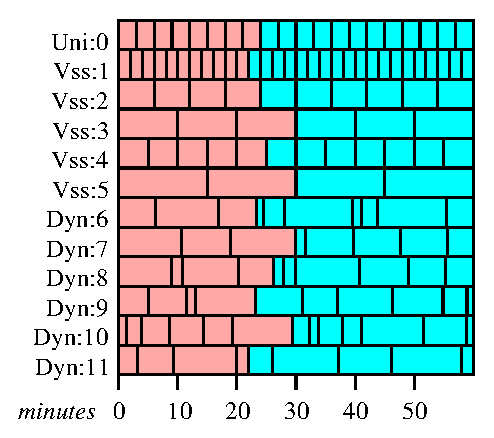
\includegraphics{Figure1}
  \caption{Time scheduling strategies.  Red boxes represent time steps that
    have already passed, blue boxes represents scheduled time steps
    that have not yet been run. ``Uni:''  and ``Vss:'' sub\-models are
    members of a uniform or variable speed splitting
    sub\-models and require uniform time steps, and ``Dyn:'' sub\-models
    have adaptive time steps.}
  \label{times}
\end{center}
\end{figure}
A better approach is the technique of variable speed splitting, such
as in \cite{walters2004fisheries} and many others. (Figure \ref{times}) This approach allows models to step through time in
different intervals by dividing the largest interval required into
smaller steps that are more appropriate for the sub\-models with
naturally shorter time scales. While models with uniform time steps are
a trivial example of this approach, variable speed splitting is almost
as simple and much more efficient.  This technique can keep the
subjective times of a set of agents moderately consistent, but ad hoc
stepping changes would still seem to be awkward or difficult.

Both of these strategies may be subject to artifacts arising from the
sequence in which agents are given their time step.  The general class
of model errors of the sort described in \cite{chivers2009generalised}
arise as a consequence of structure of the processing across the set
of agents in a simulation. \IB\ models which process agents
species-by-species will be particularly vulnerable to these sorts of
artifacts, since there will be an implicit advantage or disadvantage
to being early in the list.  Similarly, advantage or disadvantage can
arise when there is a change in rep\-re\-sen\-ta\-tion, perhaps from an
\SD\ sub\-model to an \IB\ sub\-model; a shorter time step in this
situation may introduce a great many small time steps which agents may
exploit.  This kind of problem can be overcome by introducing a
randomizing process within each time step. Early versions of the
variable speed splitting model in \cite{Lyne1994pmez5} suffered from
predator-prey artifacts arising from a na\"ive introduction of
predators and prey into the list of agents, and such randomizing was
introduced to minimize the effects. In situations where the time steps
of the interacting agents differ, implementing a randomization
strategy may require a significant increase in the complexity of the
system to accommodate irregular stepping through the lists of
agents, or a significant change in the basic structure of the model.

\cite{Gray2006nws} and \cite{Fulton2009crossingscales} describe models that have a well
developed approach to coordinating agents using adaptive time
steps. In these models agents may set their own time steps to
intervals that are suitable for their current activity or role. This
strategy can readily incorporate sub\-models with uniform time steps, or
collections that employ a variable speed splitting strategy. When
agents interact, they either explicitly become synchronous before
interaction occurs by setting their time steps appropriately and
waiting, or they implicitly acknowledge that there is a temporal
mismatch. (Figure \ref{times})

While some agents should be given execution priority (such as an agent
which models ocean currents), most agents will have their execution
order within a time step randomized, effectively preventing a large
class of execution order dependent artifacts.  The associated overhead
in the most recent work, \cite{Gray2006nws,Gray2012adaptive}, is marginally higher
than one would expect from single-stepping or variable speed stepping
systems, but the advantages arising from the ability to ensure
synchrony and change time steps in response to en\-vi\-ron\-men\-tal stimulus
outweigh the small computational overhead.  This last approach seems
likely to be the most appropriate for a general hybrid model that
supports swapping models.

General adaptive hybrid models must have a mechanism for scheduling
each agent's execution which keeps the cohort of agents roughly
synchronous, and it should able to handle changes in an agent's time
step when the agent changes its rep\-re\-sen\-ta\-tion; where possible, agents
should also be designed so that they may run at other time steps as
well as their own preferred time step so they can become synchronous
and interact at the appropriate temporal scale with other agents.

%-- MONITOR structure

\subsection{Systematically adjusting the model con\-fig\-ur\-a\-tion}
%----> Infrastructure, introduce monitor, guff about what should be in a monitor <----

A model's con\-fig\-ur\-a\-tion should only change when there is an overall
benefit in the efficiency or fidelity of the system.  A
straightforward way of determining this is to have a monitoring
routine that runs periodically, polling the agents, and ranking likely
con\-fig\-ur\-a\-tions according to their relative benefit or cost.  This
means that each sub\-model would need a way to provide, to the monitor,
a measure of its current suitability, and to indicate what it needs
from other niches. 


%---- Algorithm MonAlg
\begin{algorithm}
  \caption{Basic processing pass for the monitor}
  \label{MonAlg}
  \begin{algorithmic}
    \ForAll{niches}
    \ForAll{sub\-models in the niche}
    \ForAll{agents in the sub\-model}
    \State generate agent state vector
    \State generate the sub\-model state vector
    \State \qquad note extrinsic requirements
    \EndFor
    \EndFor
    \State
    \State generate niche state vector
    \EndFor
    \State
    \State Run niche-level assessment
    \State Flag any whole of model issues
    \ForAll{candidate con\-fig\-ur\-a\-tions}
    \State Deprecate untenable con\-fig\-ur\-a\-tion
    \State Adjust for unavoidable extrinsic
    \State $\qquad$ requirements
    \EndFor
    \State
    \State Select best indicated con\-fig\-ur\-a\-tion
  \end{algorithmic}
\end{algorithm} The last step in Algorithm \ref{MonAlg} is deliberately vague. 

Algorithm \ref{MonAlg} illustrates a possible
assessment pass for a monitor, though how appropriate it may be is an
open question. Configuration ranking for the example model will be
cast in terms of evaluating an objective function based on elements of
the vector space of tree elements described in the \appendixname.

A monitor may have large number of potential candidate con\-fig\-ur\-a\-tions,
but we would like to keep the actual number quite low. The example
model described below has a global domain associated with a particular
rep\-re\-sen\-ta\-tion, along with local domains (subregions of the global
domain) which are associated with finer scale rep\-re\-sen\-ta\-tions of the
modeled entities. The set of potential candidate trees could be quite
large; in practice we reduce the number by casting the candidate trees
in a more general way -- including trees representing particularly
good rep\-re\-sen\-ta\-tions and particularly poor rep\-re\-sen\-ta\-tions: the first
to steer the con\-fig\-ur\-a\-tion toward good choices, and the second to
drive it away from poor choices. We can use the hierarchical
organisation (whole-model, niche, sub\-model, agent) to help limit our
search space, as well as the geographic context of the agents (whole-domain, local
cell, immediate-locus).

The sets of candidate trees which are associated with particular
con\-fig\-ur\-a\-tions will need to be crafted carefully as a part of the
model design. These trees reflect the modelers understanding of the
strengths and weaknesses of each of the sub\-models (or sets of
different sub\-models) which may be employed.

Exactly how a monitoring routine is integrated into the model
framework is a subjective choice best left to the team implementing
the models, but one very attractive option is to implement the monitor
as an agent in the system. This would allow the monitor to assess its
own performance and the needs of other agents with respect to its own
suitability with the option of swapping itself our for a montitor
which implements some alternative strategy. 


%-- The example model
%--- Algorithmic description of the model
\typeout{Chapter 3: The example model}
\section{The example model}

The purpose of the example model described below, is to provide a
context for a discussion of the dynamics associated with a
hypothetical simulation using this model.  The ends of the
spectrum between \SD\ models and \IB\ models are represented, and the
environment is unrealistically simple in order to keep us from being
swamped by detail. 

\begin{figure}
\begin{center}
  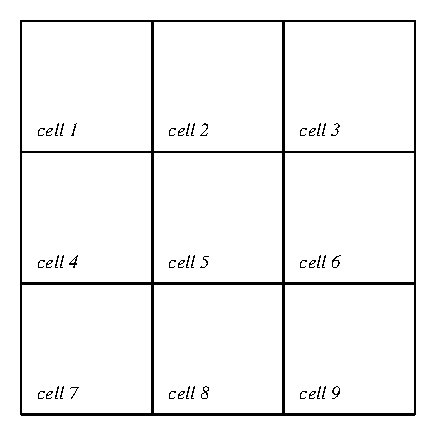
\includegraphics{Figure2}
  \caption{The model domain is divided into nine cells. An \SD\ agent
    is associated with each of these cells and with the domain as a
    whole. Any \IB\ agents which are created during the simulation
    will be associated with one cell at any given time.}
  \label{domain}
\end{center}
\end{figure}


%----> Describes phys domain, niches, food chain <----
The model consists of a spatially explicit environment that is
partitioned into nine cells (Figure \ref{domain}). The biotic elements
consist of plants, fruit, seeds, herbivores, and carnivores.  The
herbivores feed on the plants and their fruit; and carnivores prey
upon juvenile herbivores.  The plants and herbivores are
interdependent: fruit is the sole diet for juvenile herbivores and the
plants need juvenile herbivores to make the seeds viable by eating the
fruit.

%----> Introduces rep\-re\-sen\-ta\-tions of entities <----
The rep\-re\-sen\-ta\-tions are equation-based \SD\ models of the interactions
between the plants and animals and \IB\ models for plants and
animals. The \SD\ sub\-models model the biomass with respect
to size, for plants and animals, or simply numeric quantities for
fruit and seeds, and they can operate at either the global or
cell-sized scale. Modeling biomass in this way makes it possible to
minimize the loss of fidelity incurred by swapping from \IB\ agents to
\SD\ agents and visa-versa, since we preserve more of the essential
nature of the populations. A more detailed description of the
\SD\ agents is presented in the \SuppMaterial.

%----- Fruit and seeds

\subsection*{Fruit and seeds}
%------> Describes fruit and seeds <------
Fruit and seeds are treated somewhat differently to the rest of the
niches. They exist principally as numbers of entities that are updated
as a result of the activities of other, more explicit \SD\ or
\IB\ models.  There are explicit routines that deal with uniquely
``fruit'' and ``seed'' processing to handle spoilage and germination,
respectively.

For fruit and seeds we have the following relationships
\begin{equation*}
   d\N{F}(t) = \mathit{Production} - \mathit{Spoilage} - \mathit{FruitEaten}
\end{equation*}
and
\begin{align*}
  d\N{S}(t) = s &* \mathit{FruitEaten} \\
  &- \Biggl(1 - \frac{\N{P}(t)}{\K{P}}\Biggr)\mathit{Germ}.
\end{align*}
where $\N{P}(t)$ is the biomass of plants at time $t$, and $\K{P}$ is
the carrying capacity of the pertinent domain (either global or
cell-based).
%------ fruitalg
\begin{algorithm}
  \caption{Basic processing pass for fruit}
  \label{fruitalg}
  \begin{algorithmic}
    \State $\N{F} \gets \N{F} - (\mathit{Spoilage}_{\mt{F}} \cdot \N{F})$
  \end{algorithmic}
\end{algorithm}
%----- ...text continues
The processing for fruit is quite simple and consists only of
applying ``spoilage''; no reference to other agents in
the system is required, and only the number of fruit is adjusted as a
result (Algorithm \ref{fruitalg}).
%------ seedalg
\begin{algorithm}
  \caption{Basic processing pass for seeds}
  \label{seedalg}
  \begin{algorithmic}
    \State $\mathit{NewTreeCount} \gets \mathit{Germination} \cdot  \mathit{SeedCount}$
    \State $\mathit{SeedCount} \gets \mathit{SeedCount} -  (\mathit{NewTreeCount} $
    \State $\qquad + \mathit{Spoilage}_{\mt{S}} \cdot \mathit{SeedCount})$
    \State generate $NewTreeCount$ new plant agents and introduce them into the system
  \end{algorithmic}
\end{algorithm}
%----- ...text continues
Seed models will adjust their ``seed count'' as well as the biomass
distribution for plants in their time step, according to the level of
germination. Germination is probabilistic as is the size of the plant
a germinated seed becomes in its pass, though the distribution of
possibly sizes is quite restrained (Algorithm \ref{seedalg}).

%---- SD rep\-re\-sen\-ta\-tions
\subsection*{\SD\ rep\-re\-sen\-ta\-tions}

%------> desciption of animal biomass x size rep. in SD models <------
Each of the niches has an integral equation expressing the change in
biomass for a given size; an animal's equation is of the
form\footnote{See the \SuppMaterial\ for a more detailed set of
  equations.}
\begin{align*}
  d\N{A}(t,x) = & \growthnstarve + \reproduction \\
  & - \predationmort -\naturalmort.
\end{align*}

%------> no migration in SD animal models <------
We do not include migration terms in the \SD\ models, since that will
be addressed by the \IB\ forms. The assumption is that the
\SD\ rep\-re\-sen\-ta\-tion is most appropriate when population levels are
moderately high, and there is adequate food; under these conditions,
we will assume that the net migration associated with a domain will be
close to zero.

%----- Plants 
%------> desciption of animal biomass x size rep. in SD models <------
Plants are represented by similar equations, namely
\begin{align*}
d\N{P}(t,x) = &\Biggl(1 - \frac{\N{P}(t)}{\K{P}}\Biggr)[\growth + \germination] \\- \
& \predationmort - \naturalmort
\end{align*}
where $\N{P}(t,x)$ is the biomass of plants of size $x$ at time $t$.


%------> important state variables for SD models <------
The important state variables for the \SD\ are, for each domain, the
biomass-by-size distributions for plants, herbivores and carnivores, and the
raw numbers of fruit and viable seeds. 

%------ SDalg
\begin{algorithm}
  %% if we swap the order of the caption and label, we get the section number
  %% rather than the algorithm number!
  \caption{Basic processing pass for the \SD\ models}
  \label{sdalg}
\begin{algorithmic}
  \ForAll{agents in this domain}
    \State{Incorporate quantities that are }
    \State{$\qquad$ controlled in \emph{other} agents}
    \State{Run Runge-Kutta4}
    \State{Update only quantities that are}
    \State{$\qquad$ controlled by \emph{this} agent}
  \EndFor
\end{algorithmic}   
\end{algorithm}

%----- ...text continues

%------> Processing of SD models, justification of non-controlled niches <------
The system of equations described in the \SuppMaterial\ is evaluated
using a fourth order Runge-Kutta algorithm; the numbers of fruit and
seeds, and both the global and cell-based biomass distributions for
plants and animals are updated at the end of the calculation. The
model will adjust the values in the global and cell-based models to
allow data from models running with better resolution (usually more
localized models) (Algorithm {\ref{sdalg}}) to take precedence.

%------> We haven't nailed parameters down, because. <------
Most of the important parameters and many of the functions associated
with the life history of the modeled entities are not specified. This
way we may consider possible trajectories without being tied to a
particular conception or parameterization of the system.


%---- IB rep\-re\-sen\-ta\-tions
\subsection*{\IB\ rep\-re\-sen\-ta\-tions}
%------> introduction of the IB rep, follows Gray2012adaptive <------
Individual-based rep\-re\-sen\-ta\-tions for plants, herbivores and carnivores
follow the pattern in \cite{Little2006nws}; fruit and seeds are only
modeled in the \SD\ rep\-re\-sen\-ta\-tion, though their numbers are modified
by the activities of the herbivores irrespective of how those
herbivores are represented. 

\subsection{\IB\ Plants}

%------> Basic  plant state and dynamics <------
Plants maintain a reference to their cell, their location, a mass and
a peak mass.  If a plant's mass drops below a certain proportion
($\ttt{P}_{M\Omega}$) of its peak mass, it dies --- this provides a
means for the herbivores to drive the plant population to local
extinction. 

%------> sigmoidal growth rate <------
We will suppose that plants grow according to a sigmoidal function with
some reasonable asymptote and intermediate sharpness; fruiting
occurs probabilistically as in the \SD\ represen\-tation.

%------ plantalg
\begin{algorithm}
  \caption{Basic processing pass for plants}
  \label{plantalg}
  \begin{algorithmic}
    \If {$(\mass \ge \Mtt{P}_{\mature}) \land (\ttt{P}_{\fruits} \ge \Urnd)$}
    \State $\AddFruit{\ttt{P}_\rho}{\mass^{\frac{2}{3}}}$
    \EndIf
    \If {$(\mass\le\Mtt{P_{M\Omega}}\,\peakmass)\lor(\imort{P}<\Urnd)$}
    \State \Die
    \Else
    \State $\mass \gets \Gamma_{\mt{P}}(\delta t, \mass)$
    \If {$\mass > \peakmass$}
    \State $\peakmass \gets \mass$
    \EndIf
    \EndIf
  \end{algorithmic}
\end{algorithm}

%------> Describe parameters/variables <------

The plant agent goes through the steps in Algorithm {\ref{plantalg}} in each
of its time steps. In the algorithm, $\Gamma_{\mt{P}}(\delta t, mass)$ is an
analogue of the probability of a plant growing from one size to another from
the \SD\ rep\-re\-sen\-ta\-tion, $\ttt{P}_{\mature}$ is the parameter that indicates
the mass a plant must be before it fruits, $\ttt{P}_{\fruits}$ is the
probability of a mature plant fruiting, and $\ttt{P}_\rho$ is the amount of
fruit relative to the fruiting area. The routine \textsc{AddFruit} updates the
models representing fruit in the domain.

\subsection{\IB\ Animals}

%------> Basic  plant state and dynamics <------
Like the plants, animals maintain a reference to their cell, their
location, and a mass. They also maintain several variables that are
associated with foraging or predation, namely the amount of time until
they need to eat ($\satedtime$), and the amount of time they have been
hungry ($\hungertime$).

Animals will grow while they do not need to eat and will only forage
when they are hungry.  Reproduction happens in a purely probabilistic
way once the animal is large enough, and the young are not cared for
by the parents.

Animal movement is constrained so that they will tend to stay within
their nominated home cell, only migrating (changing their home cell to
an adjacent cell) when food becomes scarce or if the population
exceeds some nominated value and causes crowding.

%------> Growth, starvation and differences w.r.t. SD model <------
The analogues of the mechanisms for growth and starvation in the
\SD\ rep\-re\-sen\-ta\-tion are quite different to those of the \IB\ version.
In the \SD\ models, starvation and growth occur as a result of the
relative population levels of the consumer and the consumed rather
than the local availability of food.

%------> Animals are all the same, really, just initial setup and prey differences <------
There are no real programmatic differences between the
\IB\ rep\-re\-sen\-ta\-tions of herbivores and carnivores; their differences
lie in their choices of food and the way their ``time-to-eat''
variable is initially managed. In\-Di\-Vidu\-Al-based, new-born carnivores
begin with a long time till they need to eat. This reflects a reliance
on some unmodeled foodstuff until they are large enough to prey on
the juvenile herbivores.  In contrast, the juvenile herbivores must
begin eating fruit immediately, and only switch to foraging on plants
when they are larger (but before they can reproduce). For both
species, if the amount of time they have been hungry exceeds a
particular value, $H_\Omega$ or $C_\Omega$, the in\-di\-vidu\-al dies.

%------ animalalg
\begin{algorithm}
  \caption{Basic processing pass for herbivores and carnivores}
  \label{animalalg}
  \begin{algorithmic}
  \If {$(\imort{A} > \Urnd) \lor (\hungertime \ge \ttt{A}_\Omega)$}
  \State \Die
  \EndIf
  \State $\preylist \gets \PreyPresent{A}{\location}{\mass}$
  \If {$\satedtime \ge 0$}
  \State $\mass \gets \mass + \Growth{A}{mass}{\delta t}$
  \ElsIf {$(\hungertime \ge 0)\land(\lcount{\preylist} > 0)$}
  \State $\satedtime \gets \Eat{\preylist}{\ttt{A}_{EatLimit}}{mass}$
  \State $\hungertime \gets 0$
  \State $\foragecount \gets 0$
  \ElsIf {$(\hungertime \ge 0) \land len(\preylist) = 0)$}
  \State \textsc{Forage}
  \State $\foragecount \gets \foragecount + 1$
  \ElsIf {$(\hungertime \ge \ttt{A}_{moveT}) \lor \LocallyCrowded{A}$}
  \State $\Migrate{A}{\location}$
  \Else
  \If {$(mass \ge \ttt{A}_{RepSize}) \land (\ttt{A}_{RepP} \ge \Urnd)$}
  $\Reproduce{A}{\location}$
  \EndIf
  \EndIf
\end{algorithmic}
\end{algorithm}
%----- ...text continues

%------> effect of different parameters i.t.o. behavior <------
So, if we take \ttt{A} to represent either carnivores (\ttt{C}) or
herbivores (\ttt{H}) below, then the processing pass for an animal is
shown in Algorithm \ref{animalalg}, where $\ttt{A}_{moveT}$ is the
amount of time an animal can be hungry before it migrates,
$\ttt{A}_\Omega$ is the amount of time it takes for the animal to
starve, $\ttt{A}_{EatLimit}$ is the most the animal can eat as a
proportion of its mass, $\ttt{A}_{RepSize}$ is the minimum size an
animal may breed at and $\ttt{A}_{RepP}$ is the probability of
reproducing. The routines $\mathsc{PreyPresent}_{\Mtt{H}}$ and
$\mathsc{Eat}_{\Mtt{H}}$ have different cases for juvenile and adult
herbivores, since juveniles prey upon fruit, and the seeds from the
fruit they eat need to be accounted for in the appropriate places. There is
a similar issue with juvenile carnivores. Their \emph{preylist} will
always be set to a value that indicates that they may eat as much as
they like, and the corresponding call to $\mathsc{Eat}_{\Mtt{C}}$ will
handle this value appropriately.


%--- MONITOR: Model dynamics in the example
\subsection{The monitor and model dynamics}
%-------> commands <--------
%% {repset}{sn}
\newcommand{\cst}[1]{\node{\check{\tau}}^\Sigma_{#1}} % candidate tree 
                                                       % for config
\newcommand{\domt}[1]{\node{\check{\tau}}^\Sigma_{#1}} % candidate
                                                     % tree for a domain



%% {t}
%% {id} {t}
%% {rep} {id} {t}
%% {rep} {t}
\newcommand{\stmA}[1]{\node{\tau}^\Sigma_{#1}} % the aggregate whole model status tree at $t$
\newcommand{\stsdA}[2]{\node{\tau}^\Sigma_{SD(#1),#2}} % the aggregate cell status tree 
\newcommand{\stibA}[2]{\node{\tau}^\Sigma_{IB(#1),#2}} % the aggregate
                                                     % cell status
                                                     % tree for types
                                                     % of  individuals
%\newcommand{\nstaA}[3]{\node{\tau^\Sigma}_{(#2),#3}\vert_{#1}} % niche status tree
\newcommand{\stm}[1]{\node{\tau}_{#1}} % the whole model status tree 
\newcommand{\sta}[3]{\node{\tau}_{\ms{#1}(#2),#3}} % generic st tree
\newcommand{\stsd}[2]{\sta{SD}{#1}{#2}} % SD st tree
\newcommand{\stib}[2]{\sta{IB}{#1}{#2}} % IB  st tree
\newcommand{\staR}[3]{\node{\tau}_{\ms{#1}(#2),#3}} % generic st tree
\newcommand{\nstaR}[2]{\node{\tau}_{#1,#2}} % niche status tree at t
\newcommand{\nsta}[3]{\node{\tau}_{#1(#2),#3}} % niche status tree
\newcommand{\asta}[3]{\node{\hat{\tau}}_{\ms{#1}(#2),#3}} % alternate 

\newcommand{\stbr}[2]{\child({#1},\mc{#2})}

\newcommand{\gtentry}[4]{{#1} & {#2} & {#3} & {#4}\cr}
%\AsdGtentry{t}{txt}
\newcommand{\AsdGtentry}[2]{{#1} & \stmA{#1} & global \SD & global state in aggregate #2\cr}
%\AsdGtentry{t}{cellnum}{txt}
\newcommand{\AsdLtentry}[3]{{#1} & \stsdA{#2}{#1} & \SD: cell #2 \SD &  characterizes cell #2 in aggregate #3\cr}
%\sdGtentry{t}{txt}
\newcommand{\sdGtentry}[2]{{#1} & \stm{#1} & global \SD & global state #2\cr}
%\sdLtentry{t}{cellnum}{txt}
\newcommand{\sdLtentry}[3]{{#1} & \stsd{#2}{#1} & \SD: cell #2 \SD & characterizes cell #2 #3\cr}
%\ibtentry{t}{id}{rep}{txt}
\newcommand{\ibtentry}[4]{{#1} & \stib{#1}{#2} & \IB: #3 & {#4}\cr}


%------> table of items prompting changes <------
The following may be typical of the types of situations that could or
should cause changes in the con\-fig\-ur\-a\-tion:
\begin{itemize}
  \item \emph{Low population} ---- If, in an \SD\ representa\-tion,
    the number of in\-di\-vidu\-als filling a niche (either explicitly taken
    from a distribution, or estimated using a mean and a biomass)
    drops below a nominated value, then the biomass in that niche
    should be converted to \IB\ agents representing those
    in\-di\-vidu\-als. This type of change is motivated by the observation
    that at low population levels the assumption that we can treat the
    population as having uniform access to resources (or be uniformly
    available to predators) breaks down;

  \item \emph{High population} ---- If a niche in a cell is
    represented by \IB\ agents and the number of in\-di\-vidu\-als exceeds a
    (higher) nominated value, the biomass those agents represent
    should be subsumed by the distribution in the local
    \SD\ submodel. The change in rep\-re\-sen\-ta\-tion is attractive here for
    two reasons: an equation-based rep\-re\-sen\-ta\-tion will be much faster,
    and \SD\ submodels are arguably simpler to calibrate;

  \item \emph{Starvation risk} --- If the mean amount of time an
    animal in a cell spends \emph{hungry} in a cell exceeds half of
    $\ttt{A}_\omega$ (or some other nominated time), the prey biomass
    must convert to \IB\ agents if it isn't already so (bearing in
    mind that this isn't pertinent for fruit). This mean is calculated
    by averaging the means of each animal in the cell. If this is
    triggered, it indicates that the biomass of the prey species is
    sparse enough that homogeneity assumption is unlikely to hold;

  \item \emph{Relative biomass} --- If the biomass available for
    predation is represented in a local \SD\ agent and its density
    drops below some proportion of the minimum required to support the
    predators in the domain, the prey species should convert its
    biomass into \IB\ agents and, if the predator is represented by a
    \SD\ agent, it should also convert to an \IB\ form. If the
    biomasses are such that the effective predation rate is
    unsustainable, the mixing assumption is unlikely to hold.
\end{itemize}

%------> description of the items in the change table <------
The pertinent data for conditions will be periodically reported to the
monitor through a set of status trees. The trees are able to represent
single entities, nested entities and aggregates equally well, and can
preserve structural information which may also be used in the
comparison of these trees.  One of the basic elements we can easily
incorporate into a sub\-model's status tree is the agent's own
assessment of its competence relative to its state-vector and its
local conditions. This measure of ``self-confidence'' can probably be
maintained at little computational cost for most agents, and may be
the most significant component in a monitor's assessment. The
\emph{high} and \emph{low} population level conditions can clearly be
determined by the agent in question; it can set its level of
self-confidence upward or downward as appropriate. \emph{Starvation}
can also be encoded in the relevant node of an agent's status tree,
but since starvation alone may not indicate a problem with the way the
entity is represented, it probably wouldn't reduce the value for its
confidence.

A starvation trigger may usually arise as a natural consequence of the
population dynamics, but it may also occur when there is a mismatch in
rep\-re\-sen\-ta\-tions which has not been adequately addressed in the design
stage.  The final condition based on the relative biomasses is one
which properly lies in the realm of the monitor -- it would be quite
inefficient for each of the candidate animals to be querying their
prey for available biomass, summing the result, and then noting the
need for change.

%------> status tree types <------

The monitor will primarily use the confidence values associated with
agents and their niches, and the distance from trees which describe
the state of the model or its set of submodels to trees which describe
``known good'' con\-fig\-ur\-a\-tions. With data obtained directly from the
agents in the system and from alternative rep\-re\-sen\-ta\-tions it generates
status trees,
\begin{itemize}
\item{\qquad} $\cst{sn}$, is a candidate status tree tied to a
  specific  con\-fig\-ur\-a\-tion. The serial number, $sn$, ties it to a
  con\-fig\-ur\-a\-tion with that serial number,
\item{\qquad} $\domt{d}$, is a candidate tree which represents the
  current state of a domain,
\item[\qquad] $\stmA{t}$, an aggregate tree for the whole domain at
  time $t$,
\item[\qquad] $\stsdA{n}{t}$, aggregate trees for each cell, $n \in \{1,\ldots, 9\}$,
\item[\qquad] $\sta{R}{i}{t}$, specific status trees for each agent,
\item[\qquad] $\nstaR{R}{t}$, specific status trees for a 
  rep\-re\-sen\-ta\-tion $R$ for each rep\-re\-sen\-ta\-tion associated with a niche,
%\item[\qquad] $\nsta{R}{i}{t}$, specific status trees for 
%  rep\-re\-sen\-ta\-tion, $R$, suitable for modeling things like agent $i$
\item[\qquad] \qquad and
\item[\qquad] $\asta{R}{i}{t}$, candidate trees for all possible
  rep\-re\-sen\-ta\-tions of each agent $i$,
\end{itemize}
at the beginning of each of its steps. The model may have a mix of
\SD\ and \IB\ rep\-re\-sen\-ta\-tions, and some of the trees will have to
incorporate data from many agents ($\stmA{t}$, any of the
$\asta{R}{i}{t}$, and $\nstaR{R}{t}$, for example). A candidate tree is
a status tree which represents an alternative sub\-model in a niche, and
candidate trees are generated for specific agents and for each niche. When the
monitor begins to generate status or candidate trees for a given
agent, it first looks to see if it has generated an appropriate tree
already.  If it finds one, it incorporates or adjusts the tree
appropriately; perhaps by incorporating the agent's biomass  and size
into the tree's data.  We will also denote the con\-fig\-ur\-a\-tion of a
domain (global or local) with $\domt{c}$ where $c$ identifies the
domain in question.

The monitor assesses the trees by calculating aggregate values of
particular attributes, comparing the trees' divergences from allegedly
ideal con\-fig\-ur\-a\-tions, and by looking how uniform groups are -- groups
of in\-di\-vidu\-als that are all very similar are good candidates for
simpler rep\-re\-sen\-ta\-tions. 

We can calculate the average confidence value from any of these trees
by evaluating \[
\frac{\nabs{\nmask(\node{\tau},
    \mc{confidence},0)}}{\supp(\nmask(\node{\tau},
  \mc{confidence},0))},
\]
for example. The trees and functions to manipulate them are described
in the \appendixname.



\begin{figure}
\begin{center}
  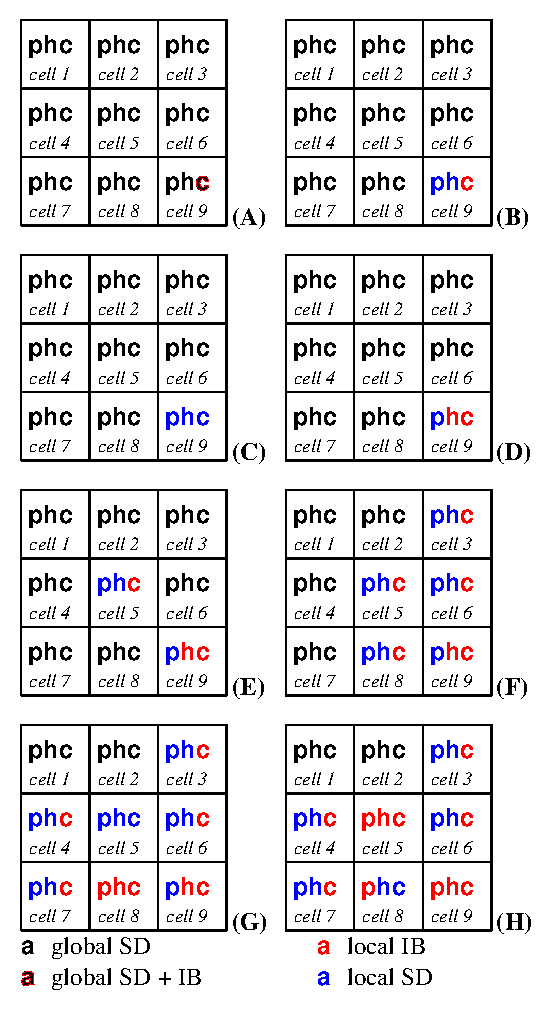
\includegraphics{Figure3}
  \caption{The color of the \textbsf{p},\textbsf{h} and \textbsf{c}
    indicate an agent's current rep\-re\-sen\-ta\-tion within a cell
    at various points in the description of a simulation.  In each, a
    black symbol indicates that the biomass of plants (\textbsf{p}), herbivores
    (\textbsf{h}) or carnivores (\textbsf{c}) is modeled with the global \SD\ agent, a
    blue symbol indicates that the biomass is modeled with a cell's
    \SD\ agent, and red indicates that an \IB\ model is being
    used. Symbols composed of two colors indicate that more than one
    rep\-re\-sen\-ta\-tion is currently controlling portions of the
    relevant biomass.}
  \label{timeline}
\end{center}
\end{figure}

%------> walking through the  <------
Now let us consider what a simulation might look like. Figure
\ref{timeline} provides an overview of the con\-fig\-ur\-a\-tion of the system
as our hypothetical simulation runs. The model begins with eleven
agents (not counting the monitor). The monitor runs its first step
generating the status trees: $\stmA{0},$ which characterizes the model
in aggregate, $\stsdA{0}{0},\ldots,\stsdA{9}{0},$ which record the
aggregate state of the ten \SD\ submodels, the aggregate status tree for
the \IB\ agent, $\stibA{0}[9]$, status trees for the \SD\ submodels:
$\stsd{0}{0}$--$\stsd{10}{0}$, the status tree for the lone carnivore,
$\sta{\IB}{11}{0}$, followed by the trees which represent alternative
agents: $\asta{\SD}{0}{0}$--$\asta{\SD}{10}{0}$ and
$\asta{\IB}{11}{0}$.  As mentioned earlier, there is only the single
tree for agent 11 (the carnivore) since its alternative rep\-re\-sen\-ta\-tion
is embodied in $\asta{\SD}{10}{0}$. During the simulation a simulated
fire will occur.

The first steps which must be taken before ranking of potential
configur\-ations is to find the sets of candidate trees which best
approximate the current con\-fig\-ur\-a\-tion at both the global and
cell levels. We do this by calculating a similarity index or a
distance which indicates how close each of the candidate trees are to
the configur\-ation of each of the domains. There are many ways we
could do this: for an index which only considers structural similarity
we might use something like the simple function
\begin{equation*}
  \ssim(\node{c},\node{\tau_d}) =
  \frac{\overlap(\node{c},\node{\tau_d})}{\max(\Tcard{c},\Tcard{\tau_d})}, 
\end{equation*}
but for a more comprehensive treatment which factors values which are
incorporated into the candidate and status trees we might apply the
$\devi{}{}$ or $\dist{}{}$ functions described in the \appendixname. The
$\dist{}{}$ function is a well-defined distance over the vector space of
trees, while the $\devi$ function is an index of similarity that
incorporates structural characteristics as well as the numerical
distance between compatible subtrees.  To refine such an analysis we could apply
$\mask$ and $\nmask$ to select only the relevant parts of the
candidate and status trees.

So to assess the con\-fig\-ur\-a\-tion of a domain, we would use our chosen
measure to construct a set of the results of applying an optimisation
function, $opt$, to each of the candidate trees and their similarity
to the current con\-fig\-ur\-a\-tion.  So if $\set{S}$ is the set of all
serial numbers for candidates, $\domt{d}$ is the status tree fo the
current domain, and  is the  , we calculate
\begin{equation*}
  \set(C) = \{(\delta(\domt{d},\cst{i}),i): \forall i \in \set{S}\},
\end{equation*}
and this is used to generate
\begin{equation*}
  \set{C}^* = \{(\opt(\cst{i}),c,\cst{i},i): \forall(c,i) \in \set{C}\}
\end{equation*}
where $\delta$ stands for our chosen measure of similarity.

\begin{figure}
\begin{center}
  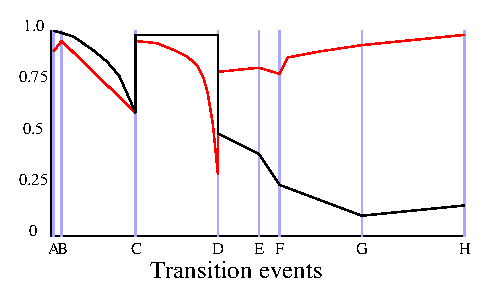
\includegraphics{Figure4}
  \caption{Normalized indexes of execution speed (black) and fidelity (red) the 
    against configuration changes through time associated with Figure \ref{timeline}}
  \label{indices}
\end{center}
\end{figure}

The elements in $\set{C}^*$ are then assessed by the monitor, and the
best permissible candidate is selected. If there is only a small
improvement on the current con\-fig\-ur\-a\-tion, $\domt{d}$, the monitor will
leave the con\-fig\-ur\-a\-tion as it is; otherwise, the monitor would then manage
the creation of new agents to replace less optimal rep\-re\-sen\-ta\-tions and
manage the exchange of state data. 




So the early phase of our simulation might begin like so:

\begin{enumerate}
\item %A
Both of the aggregate trees $\stmA{0}$ and $\stsdA{9}{0}$ indicate
that there is an \IB\ agent in their domain and that their
\SD\ rep\-re\-sen\-ta\-tion does not perform well for the indicated
biomass. Both the status and candidate trees for agent 11,
$\staR{11}{0}, \nsta{\IB}{11}{0}$ and $\asta{\IB}{11}{0}$, indicate
that it is confident that it can represent the biomass, and that there
are no immediate unmet requirements from other agents.  Figure 
\ref{timeline} (\textbf{A})

\item %B
%-------> Finding a match <--------
The monitor assesses the trees against a prepared set of
con\-fig\-ur\-a\-tions: each of the alternative con\-fig\-ur\-a\-tions (including the
current con\-fig\-ur\-a\-tion) is compared to a set of prepared, ``efficient''
con\-fig\-ur\-a\-tions.  The con\-fig\-ur\-a\-tion of cell 9, $\domt{9}$, notes
global \SD\ rep\-re\-sen\-ta\-tions for plants and herbivores. This
con\-fig\-ur\-a\-tion is ranked lower than the alternative which has an
in\-di\-vidu\-al based model for carnivores and a local \SD\ submodel for the
other entities in the cell.   The monitor makes this change in con\-fig\-ur\-a\-tion,
and informs the global \SD\ agent that it is no longer controlling the
biomasses in cell 9. Figure
\ref{timeline} (\textbf{B}) \label{firstconv}

\item %C
\label{cv1}
%-------> Run for a while and convert C to SD <--------
The model may run for some time without any change in con\-fig\-ur\-a\-tion.
Both the herbivores and carnivores breed. The increased execution speed
between \textbf{C} and \textbf{D} in Figure \ref{indices} is a result
of a change in representation: the number of
carnivores, recorded in $\stsdA{C}{t_4}$, reaches a point that prompts
the monitor to convert them to an \SD\ form.
Figure \ref{timeline} (\textbf{C})

\item %D
%-------> Run for a while, herbivore population drops  <--------
The biomass of carnivores has increased significantly by the time the
model reaches \textbf{D} in Figure \ref{indices},
and they are now eating all the young herbivores; as a result the
carnivore population is now prey-limited, and the \emph{Relative
  biomass} condition is triggered.  Both the carnivore and herbivore
populations are converted to \IB\ rep\-resentations. Notice that
dynamics in the fidelity in Figure \ref{indices} around \textbf{D}
arise from the collapse of the carnivore's prey, followed by the
increase in fidelity after the representation change at \textbf{D}.
Figure \ref{timeline} (\textbf{D})

\item %E
%-------> + monitor converts cell 5 in fashion analogous to start  <--------
A carnivore, agent 43, has been hungry ($(\hungertime \ge
\ttt{A}_{moveT}$) and has migrated to the cell 5
(noted in $\sta{\IB}{43}{t_5}$). As occurred in cell 9 at step \ref{firstconv}, the monitor
converts plants and herbivores in cell 5 to a local
\SD\ rep\-re\-sen\-ta\-tion, with \IB\ carnivores. Figure \ref{timeline}
(\textbf{E})

\item %F
%-------> H biomass still too large w.r.t C, but C is hungry #2 %<--------
A lot of activity has occurred in this monitor interval: 
a \emph{Starvation risk} is triggered in cell
9 because too many of the carnivores are hungry (many of the
$\sta{\IB}{n}{t_7}$ trees indicate that the elapsed time without eating is
greater than $\hungertime$). There has been more migration to
cells 5,6 and 8 from cell 9 (more of the $\sta{\IB}{n}{t_7}$ trees
indicate residence in new cells), and a chance migration has introduced a
carnivore into cell 3 from cell 5. Cells 3,6 and 8 are converted to
local \SD\ and \IB\ rep\-re\-sen\-ta\-tions as happened in step
\ref{cv1}. Figure \ref{timeline} (\textbf{F})

\item %G
%-------> cell 9: C pop crashes <--------
The population of carnivores in cell 9 crashes as a result of
migration and the scarcity of prey, (reported in $\domt{9}$) The
\IB\ juvenile herbivores are patchy and harder to find, so only a few
carnivores are getting enough to eat. There will be many
$\sta{\IB}{n}{t_{10}}$ which indicate hunger or death due to
starvation. The monitor cleans up the dead agents.  There are chance
migrations from cell 5 into cells 4 and 7 (in $\stsdA{4}{0}$ and
$\stsdA{7}{0}$). A fire begins in cell 8, moving through cell 5:
biomass loss in all niches causes all niches to shift to
\IB\ rep\-re\-sen\-ta\-tions. Figure \ref{timeline} (\textbf{G})

\item %H
%-------> cell 9: Hj begins to appear, but P biomass converts (\#3) <--------
Juvenile herbivores are reappearing in cell 9, but the available plant
biomass (recorded in $\stsd{9}{t_{11}}$) has dropped due to reduced
germination rates, triggering the \emph{Relative biomass} condition in
cell 9 causing the plants to convert to an \IB\ rep\-re\-sen\-ta\-tion.  The
fire in cell 8 has killed all animal biomass in the cell; they
\emph{do not} return to the global \SD\ rep\-re\-sen\-ta\-tion because their
status trees diverge by too much.  Instead, they convert to local
\SD\ rep\-re\-sen\-ta\-tions (which represent zero biomass quite
efficiently). Plants remain as \IB\ agents The fire spreads to cell
5. Figure \ref{indices} shows a modest increase in execution speed
between \textbf{G} and \textbf{H} due to the population losses
associate with the fire. 
Figure \ref{timeline} (\textbf{H})

\item[$\bullet$] \ldots the simulation continues
\end{enumerate}


%-- Discussion
\typeout{Chapter 3: Discussion}
\section{Discussion}
%-----> Where do we put the smarts? <-----

Adaptive hybrid models \emph{can} be constructed so that each
submodel is aware of its other rep\-re\-sen\-ta\-tions and is able to change
form as appropriate \citep{Gray2012adaptive}. This approach requires each
model to have a reasonably close coupling with its alternative
rep\-re\-sen\-ta\-tions, and the burden of instrumenting (and maintaining) the
necessary code quickly becomes untenable in complex models.  Worse, it
removes the possibility of more subtle con\-fig\-ur\-a\-tion management that
can accept poor performance in one part of a system in exchange for
much better performance elsewhere.  It seems that a guiding principle
should be that in an adaptive hybrid model, each rep\-re\-sen\-ta\-tion should
know only as much about the rest of the model as it \emph{must} know,
and no more. The facility for a sub\-model to delve into the workings of
other sub\-models, or the workings of the model as a whole, decreases
the clarity that hybrid modeling makes possible, and opens avenues
for unwanted, unanticipated behavior.

The major argument in favor of closely integrated rep\-re\-sen\-ta\-tions for
sub\-models is that it makes common (or at least similar) state
variables easy to maintain across rep\-re\-sen\-ta\-tions, even in the face of
many rep\-re\-sen\-ta\-tion changes. It is an attractive arguement, but the
long term consequence is an ever growing burden of code maintenance.

Constructing hybrid models isn't significantly more complex than
constructing traditional models. Adaptive hybrid models of the sort
described in this paper will require a more significant investment in
the design of a monitoring routine, and in the crafting of appropriate
sets of candidate con\-fig\-ur\-a\-tions.  The transition dynamics such a
model will exhibit depend on the sets of candidate con\-fig\-ur\-a\-tions, and
it seems likely that a combination of analysis and experimentation may
be the most effective way to develop a set of useful con\-fig\-ur\-a\-tions.
The hybrid models associated with \cite{Lyne1994pmez5, Little2006nws,
  Fulton2009crossingscales} were built by extending the repertoire of ways of
representing elements of the ecosystem or the anthropic components
rather than wholescale redesign and replacement.

We can imagine an ideal adaptive hybrid model, where any state
information which must be passed on is accompanied by an appropriate,
opaque parcel of code to perform the maintenance. As long as the
monitor knows what information each of these maintenance interfaces
needs, they can be updated each time the monitor interrogates the
agent which has control of the state data.  This is a readily
attainable ideal: many programming languages support first class
functions with closures, and these features are precisely what we need
to address this problem.  \textsl{Scheme, Python, ML, Common Lisp,
  Lua, Haskell}, and \textsl{Scala} all have first order functions
with closures and, hence, the capacity to build model systems with this
capability.

The state vectors and their supporting maintenance procedures can be
treated as data and passed in lists associated with the status
trees. If a monitor decides to swap rep\-re\-sen\-ta\-tions, the accumulated
lists of maintenance functions may be passed on to the new
rep\-re\-sen\-ta\-tion.  A new rep\-re\-sen\-ta\-tion inherits a maintenance list with
variables that are part of its native state, it can claim them as its
own and continue almost as though it had been running the whole
time. In this way, a new rep\-re\-sen\-ta\-tion doesn't need to know anything
about its near kin, only that it must be able to run these black-box
functions that come from other sub\-models, and to pass them on when
required.

It may seem that this concentrates the global domain knowledge in the
monitor, but this is not really the case.  The monitor knows how to
blindly query agents for state data and to the data in maintenance
procedures. The monitor also knows how to recognize and rank
characterizations of the states of the submodels or niches and to use
those data to select a con\-fig\-ur\-a\-tion.

The domain knowledge is encapsulated in the sets of targets the
monitor matches the current con\-fig\-ur\-a\-tion against, and in the
heuristic triggers (such as \emph{Starvation risk}) associated with a
sub\-model or niche.

The essential problems any monitor is likely to deal with are
problems of set selection (recognition, pattern matching\ldots) and
optimisation.  These are common tasks: web searches, voice
recognition, and route planning have become ingrained parts of modern
society. Like route planning, the monitor needs to be able to reassess
the ``optimal'' strategy as an ongoing process.

%----> decision trees,NN,BN,SVM, example uses trees  <----

There are many options to choose from to rank con\-fig\-ur\-a\-tions. A few of
the likely candidates include
\begin{itemize}
  \item using an objective function to evaluate each of the possible
    con\-fig\-ur\-a\-tions,
  \item selecting a con\-fig\-ur\-a\-tion based
    on decision trees,
  \item
    using neural nets to match model states and direct
    us to an appropriate con\-fig\-ur\-a\-tion,
  \item using Bayesian networks to determine the most likely
    candidate,
  \item[and]
  \item using support vector machines to select the
    target/con\-fig\-ur\-a\-tion pairs.
\end{itemize}

In writing this paper, one of the vexing difficulties has been finding
a suitable math\-e\-mat\-i\-cal rep\-re\-sen\-ta\-tion which would allow comparisons
between con\-fig\-ur\-a\-tions, sub\-model states and the states of niches.  We
need proxies that describe models and con\-fig\-ur\-a\-tions of models in a
way that we may readily understand, manipulate and reason about, and
being able to deal with sub\-models which are, in themselves, adaptive
hybrid models, seems to be a naturally desirable trait.  The vector
space of trees described in the \appendixname\ has some nice
properties, and may be directly useful with many of the options above:
it forms a commutative ring (without necessarily having a unit), and
would naturally inherit the body of techniques which only require the
properties of such a ring.

%-- Conclusion
\typeout{Chapter 3: Conclusion}
\section{Conclusion}

There are still some major obstacles to developing a fully fledged
adaptive hybrid model which is generic enough to tackle instances as
varied as marine ecosystem modeling and urban planning. Foremost is a
relative lack of real examples.  The simulation of the hypothetical
model\footnote{The model described in this paper is currently under
  development and will be made freely available when it has been
  completed.}  has tried to expose the character of an adaptive hybrid
model which uses a monitor to manage the con\-fig\-ur\-a\-tion of the system.
There are parts of the description of the example system which are
conspicuous by their absence; this is largely because they lie in
almost wholly uncharted water.  As a modeling community, we need to
develop a wide range of approaches to how a model may assess the
relative merits of a set of con\-fig\-ur\-a\-tions. Many of the mechanisms we
need for adaptive hybrid models already exist, but are found in domain
specific models, and in wholly different domains, such as search
engines and GPS navigation.

Establishing a suitable math\-e\-mat\-i\-cal represen\-tation for model
con\-fig\-ur\-a\-tions which gives us access to well developed techniques for
set selection, pattern recognition and component analysis would seem
to be almost as urgent as adaptive hybrid examples of real systems.


\noindent\emph{Acknowledgments}\linebreak
The authors would like to thank two anonymous reviewers whose comments
have improved the paper immeasurably.  Thanks also go to a patient and
understanding editor at Frontiers, and to Dr Tony Smith, who gave up a
weekend to work a scientifically and grammatically fine toothed comb
through the paper.  The responsibility for any mistakes, awkward
sentences, or places where it just does not make sense now rests
completely with the lead author.


%-  Bibliography

%\bibliography{biblio}
%%\bibliographystyle{frontiersSCNS}
%\bibliographystyle{plain}

%- Appendices

%\appendix


%-- Appendix: Mathematical section

%% The mathematics formats poorly in two column mode.
\onecolumn

\typeout{Chapter 3: \appendixname}
\section{\appendixname}
\subsection{Mathematical definitions}
\label{AppTrees}
The trees we use are members of a normed vector space: we can add
them, find out how far apart they are and interpolate between them. In
principle, we can run clustering algorithms to find con\-fig\-ur\-a\-tions
that are similar, and identify when a model has left one cluster and
entered another.

%--- Preliminary definitions

%---- Domain 
\begin{definition}
  \label{defdomain}
  Let $\mc{S}$ be a set of labels, and let \TFIELD\ be a field like
  the real or complex numbers. Then we define a node $\node{n}$ as a
  triplet of the form $(\mc{s}, v, \set{E})$, with $v \in \FIELD$,
  $\mc{s} \subset \mc{S}$, and the set $\set{E}$ is a (possibly empty)
  set of nodes of the same form with the restriction that no two nodes
  in $\set{E}$ may have the same label in their first ordinate.  We
  also define the triple $\nulltree = (\emptyset, 0, \emptyset)$,
  which we will call the null tree, and define \TDOM\ to be the union
  of the set of all trees composed of a finite number of these nodes.

  The ordinates of $\node{u} = (\nlabel{u}, \nv{u}, \extn{u})$ in
  \TDOM\ correspond to its \emph{label}, \emph{value}, and
  \emph{extension set}.  An element of $\extn{u}$ will be called an
  \emph{extension}.
\end{definition}


%---- Terms 
In our discussion, it will help to have a few more descriptive terms.

A node with an empty extension set is called a \emph{simple}
node, if this node happens to be a root node, then it is a simple tree.

Two trees, $\node{u}, \node{v} \in \DOM$ are called
  \emph{compatible} if either $\nlabel{u} = \nlabel{v}$ or at least
  one of \tnode{u} and \tnode{v} is \tnulltree.

We define the \emph{depth} of a tree with:
  \begin{align*}
    \depth(\node{u}) = \begin{cases}
      0 & \text{ if } \node{u} = (\emptyset,0,\emptyset) = \nulltree \\
      1 & \text{ if } \node{u} \text{ is a simple node} \\
      1 + \max(\lbrace\depth(\node{v}):\forall \node{v} \in \extn{u}\rbrace) & \text{otherwise.}
    \end{cases}
  \end{align*}

We will also define for \(\node{u} \in \DOM\),
  \begin{align*}
    \trim(\node{u}) = \begin{cases}
      \nulltree & \text{ if } \node{u} = \nulltree \\
      \nulltree & \text{ if } \node{u} \text{ is simple} \\
      (\nlabel{u}, \nv{u}, \lbrace \trim(\node{e}): \\
      \qquad\qquad\forall\node{e}\in\extn{u} \rbrace \setminus \{\nulltree\}) & \text{otherwise.}
    \end{cases}
  \end{align*}

The cardinality of a tree is the number of nodes it
  contains. Specifically, 
  \begin{align*}
    \Tcard{\node{u}} = \begin{cases}
      0 & \text{ if } \node{u} = \nulltree\ \\
      1 + \sum_{\node{e}\in\extn{u}} \Tcard{\node{e}} & \text{otherwise.}
    \end{cases}
  \end{align*}

  Simple nodes are the only nodes that have a cardinality of one, and \tnulltree\ is the only node or tree with a
  cardinality of zero.

The support of a tree is the number of nodes which have a
  non-zero value.
  \begin{align*}
    \supp(\node{u}) = \begin{cases}
      0 + \sum_{\node{e}\in\extn{u}} \supp(\node{e}) & \text{ if } \nv{u} = 0 \\
      1 + \sum_{\node{e}\in\extn{u}} \supp(\node{e}) & \otherwise.
    \end{cases}
  \end{align*}

Related is the fundamental support of a tree, which only counts nodes
with no zero valued nodes in their connection to the root node
  \begin{align*}
    \fund(\node{u}) = \begin{cases}
      0 & \text{ if } \nv{u} = 0 \\
      1 + \sum_{\node{e}\in\extn{u}} \fund(\node{e}) & \otherwise.
    \end{cases}
  \end{align*}
  Clearly the support of a tree, $\supp{\node{u}}$,  must lie in the
  domain $[0,\Tcard{\node{u}}]$ and $\fund{\node{u}} \le \supp(\node{u})$.


The \emph{overlap} between two trees is defined
  \begin{align*}
    \overlap(\node{u},\node{v}) = \begin{cases}
      0 & \text{ if } \node{u} = \nulltree \mor \node{v} = \nulltree \mor \nlabel{u} \neq \nlabel{v} \\
      1 + \displaystyle\sum_{\substack{\node{e}\in\extn{u} \\ \node{f}\in\extn{v}}} \overlap(\node{e},\node{f}) & \text{otherwise}
    \end{cases}
  \end{align*}

  Clearly two trees, \tnode{u} and \tnode{v}, are compatible if and only if \(\overlap(\node{u},\node{v}) \neq 0 \) ; they will
  be said to \emph{completely overlap} if \(\Tcard{\node{u}} = \Tcard{\node{v}} =
  \overlap(\node{u},\node{v})\).


%--- Scalar multiplication 

We can now define scalar multiplication, and tree addition.
\begin{definition}
  \label{defscalar*}
  Take $a \in \FIELD$ and $\node{u} \in \DOM$, then
  \begin{equation}
    a\node{u} = \begin{cases}
      %%      \nulltree & \text{if } a = 0 \mor \node{u} = \nulltree \\
      \nulltree & \text{if } \node{u} = \nulltree \\      
      \bigl(\nlabel{u}, a\nv{u}, \{a\node{f}: \node{f} \in \extn{u}\}\setminus\{\nulltree\}\bigr) & \text{otherwise.}
    \end{cases}
  \end{equation}
\end{definition}



%--- Tree addition

\begin{definition}
  \label{deftree+}
  Let $\node{u}$ and $\node{v}$ be compatible elements of \TDOM. Then taking the
  symbol $+$ to be addition in the field \TFIELD, we extend  it to addition in
  \TDOM\ so that for nodes \tnode{u} and \tnode{v},

  \begin{align}
    \node{u}+\node{v}=\begin{cases}
    \nulltree & \text {if } \node{u} = \node{v} = \nulltree \\
    %%!    \nulltree & \text {if } \extn{u} = \extn{v} = \nulltree \mand \nv{u} = \nv{v} = 0 \\
    %% we don't really want to loose the data associated with the labels --- zero is a valid number after all 
    \node{u} & \text {if } \node{u} \neq \nulltree \mand  \node{v} = \nulltree \\
    \node{v} & \text {if } \node{u} = \nulltree \mand \node{v} \neq \nulltree  \\
    (\nlabel{u}, \nv{u} + \nv{v}, \emptyset) & \text{if } \extn{u}, \extn{v} = \emptyset \\
    \Bigl(\nlabel{u}, \nv{u} + \nv{v}, \bigl(\{\node{f}+\node{g}:\node{f}\in\extn{u}\mand\node{g}\in\extn{v}\mand\nlabel{f}=\nlabel{g}\} & \\
    \qquad\cup\{\node{f}:\node{f}\in\extn{u}\mand\nlabel{f}\neq\nlabel{g}\forall\node{g}\in\node{v}\} & \\
    \qquad\cup\{\node{g}:\node{g}\in\extn{v}\mand\nlabel{g}\neq\nlabel{f}\forall\node{f}\in\node{u}\}\bigr)\setminus\{\nulltree\}\Bigr)  & \text{otherwise.}
    \end{cases}
  \end{align}
\end{definition}

%--- Tree inner-multiplication

\begin{definition}
  \label{deftree*}
  Let $\node{u}$ and $\node{v}$ be compatible elements of \TDOM. Then 
  we define inner-multiplication between the two nodes
  \begin{equation}
    \node{u}\cdot\node{v} = \bigl(\nlabel{u}, \nv{u} \nv{v}, \{\node{f}\cdot\node{g}: \node{f} \in \extn{u},\node{g} \in \extn{v} \mand \nlabel{f} = \nlabel{g}\}\setminus\{\nulltree\}\bigr)
  \end{equation} 
\end{definition}



%--- Assert vector space, define \nabs{\node{u}}

It can be shown that \TDOM\ with scalar multiplication and tree addition forms a vector space. This
isn't quite enough to give us distances between trees, however, so we define a semi-norm
\begin{definition}
  \label{defnabs}
  Let \tnode{u} be an element of \TDOM. Then we can define a semi-norm over \TDOM
  \begin{align*}
    \nabs{\node{u}} = \begin{cases}
      0 & \text{ if } \node{u} = \nulltree \\
      \abs{\nv{u}} & \text{ if }\extn{u} = \emptyset \\
      \abs{\nv{u}} + \sum_{\node{e}\in\extn{u}}\nabs{\node{e}} & \text{otherwise.}
    \end{cases}
  \end{align*}
\end{definition}


It is clear that $\nabs{\node{u}}$ will always be non-negative, and the only shortcoming is that we
can have a node \tnode{u} with $\nabs{\node{u}} = 0, \mbut \node{u} \neq \nulltree$.  In order to turn
this into a normed vector space we take the set $\nullspace = \{\node{u}: u \in \DOM \mand
  \nabs{\node{u}} = 0\}$ and we construct an equivalence relation on \TDOM\ by the rule $[\node{u}]
\equiv [\node{v}]$ if and only if there exist $\node{z_u}, \node{z_v} \in \nullspace$ such that
$\node{u} + \node{z_u} = \node{v} + \node{z_v}$.  It can be shown that scalar multiplication,
tree addition, \blockcomment{tree multiplication,} and the semi-norm behave appropriately with
respect to the equivalence classes. This means that if we identify
elements of \TDOM\ with their equivalence class, then we can take $\nabs{\node{u}}$ to be a norm and
that it induces a distance function \[\dist(\node{u},\node{v}) = \nabs{\node{u} - \node{v}}\].

%----- Define mask and nmask

\begin{definition}
  \label{mask}
  We define the functions $\mask$ and $\nmask$ that set the values
  associated with particular nodes in a tree to $v\in\FIELD$.  Specifically,
  if $\mc{L} \subset \SDOM$, then
  \begin{equation}
    \mask(\node{u},\mc{L},v) = \begin{cases}
     (\nlabel{u}, v, \{\mask(\node{f},\mc{L},v):  \node{f}\in\extn{u}\}) & \text{ if } \nlabel{u} \in \mc{L} \\
      (\nlabel{u}, \nv{u}, \{\mask(\node{f},\mc{L},v): \node{f}\in\extn{u}\}) & \text{otherwise}
    \end{cases}
  \end{equation}
  and
  \begin{equation}
    \nmask(\node{u},\mc{L},v) = \begin{cases}
     (\nlabel{u}, v, \{\nmask(\node{f},\mc{L},v):  \node{f}\in\extn{u}\}) & \text{ if } \nlabel{u} \not\in \mc{L} \\
     (\nlabel{u}, \nv{u}, \{\nmask(\node{f},\mc{L},v): \node{f}\in\extn{u}\}) & \text{otherwise.}
    \end{cases}
  \end{equation}
  $\mask(\node{u},\mc{L},0)$ would return a tree similar to \tnode{u},
  but all its nodes that have labels in $\mc{L}$ would have values of zero.

  We also define several functions which prune or select a child from
  a tree's extension set. This function returns only the part of
  \tnode{u} which overlaps \tnode{p},
  \begin{equation}
    \excise(\node{u},\node{p}) = \begin{cases}
      (\nlabel{u}, \nv{u}, \{\excise(\node{f},\node{g}): \node{f}\in\extn{u} \mand \node{g}\in\node{p} \mand \nlabel{f} = \nlabel{g}\} \setminus \{\nulltree\}) & \text{ if } \nlabel{u} = \mc{L} \\
      \nulltree & \text{ if }  \nlabel{u} \neq \nlabel{p} \\
      (\nlabel{u}, \nv{u}, \emptyset) & \text{otherwise,}
    \end{cases}
  \end{equation}
  and this one either returns an appropriately labelled child from the extension set (a
  branch), or \tnulltree.
  \begin{equation}
    \child(\node{u}, \mc{l}) = \begin{cases}
      \node{f} & \text{ if } \nlabel{f} = \mc{l} \mand \node{f} \in  \extn{u} \\
      \nulltree & \text{otherwise.}
    \end{cases}
  \end{equation}

%%%% This is really wrong: relabel would introduce multiple nodes with
%%%% the same labels into an extn set.
  %%
  %% We also define a relabelling function $\relabel$, where the label of
  %% a node is replace with another, $\mc{l}$, if the nodes label is a member of a
  %% set of labels, $\mc{L}$
  %% \begin{equation}
  %%   \relabel(\node{u},\mc{L},\mc{l}) = \begin{cases}
  %%    (\mc{l}, v, \{\relabel(\node{f},\mc{L},\mc{l}):  \node{f}\in\extn{u}\}) & \text{ if } \nlabel{u} \in \mc{L} \\
  %%     (\nlabel{u}, \nv{u}, \{\relabel(\node{f},\mc{L},\mc{l}): \node{f}\in\extn{u}\}) & \text{otherwise,}

  %%   \end{cases}
  %% \end{equation}


\end{definition}

%--- define deviation

We now finish with a definition of a function, $\devi{}{}$, that gives us a
measure of the degree of divergence between two trees.
\begin{definition}
  \label{defdeviation}
  The degree of deviation between two trees, \tnode{u} and \tnode{v} is given  by the expression
  \begin{equation}
    \devi{\node{u}}{\node{v}} = \begin{cases}
      \Tcard{u} + \Tcard{v} - 2\overlap(\node{u},\node{v}) + \nabs{\node{u} - \node{v}}&\text{if }\node{u} \mand \node{v} \text{ are compatible} \\
      \Tcard{u} + \Tcard{v} & \text{ otherwise.}
    \end{cases}
  \end{equation}
  
  The rationale behind this definition is that if trees \tnode{u} and \tnode{v} are identical, then
  $\devi{\node{u}}{\node{v}}$ will be zero. We also want nodes that aren't common to both trees to
  count as differences.
\end{definition}
%%%\end{document}

\typeout{Chapter 3: Epilogue to the paper}
\section{Epilogue to the paper}

The model described in this paper has been used as a template for the
model discussed in Chapter \ref{explicitmodel}.
